% =============================================================================
%  GFAz poster -- T2T-F2F 2026, UC Santa Cruz
%  42 in wide x 45 in tall  (106.68 cm x 114.30 cm)
%  Build:  pdflatex poster.tex   (run twice, for QR codes)
% =============================================================================
\documentclass[final,t]{beamer}
\usepackage[size=custom,width=106.68,height=114.30,scale=1.21,orientation=portrait]{beamerposter}
\usetheme{default}
\usecolortheme{default}
\beamertemplatenavigationsymbolsempty

\usepackage[T1]{fontenc}
\usepackage{lmodern}
\usepackage{helvet}
\renewcommand{\familydefault}{\sfdefault}
\usepackage{amsmath,amssymb}
\usepackage{booktabs}
\usepackage{multirow}
\usepackage{graphicx}
\usepackage{xcolor}
\usepackage{colortbl}
\usepackage{qrcode}
\usepackage{tikz}
\usetikzlibrary{arrows.meta,positioning,fit,backgrounds,calc}
\usepackage{microtype}

\graphicspath{{figures/}}

% ---------------------------------------------------------------- palette ---
\definecolor{cherry}{RGB}{157,34,53}
\definecolor{slate}{RGB}{33,42,54}
\definecolor{teal}{RGB}{0,112,118}
\definecolor{paleg}{RGB}{243,244,246}
\definecolor{palec}{RGB}{251,238,241}
\definecolor{palet}{RGB}{232,244,244}
\definecolor{rule}{RGB}{206,211,219}
\definecolor{hdr}{RGB}{224,227,232}

% ------------------------------------------------------------------ blocks --
\setbeamercolor{block title}{bg=white,fg=cherry}
\setbeamercolor{block body}{bg=white,fg=slate}
\setbeamerfont{block title}{size=\large,series=\bfseries}
\setbeamerfont{block body}{size=\normalsize}
\setbeamercolor{structure}{fg=cherry}
\setbeamertemplate{itemize item}{\color{cherry}\textbullet}
\setbeamertemplate{blocks}[rounded][shadow=false]
\setbeamersize{text margin left=0mm, text margin right=0mm}
\setlength{\leftmargini}{1.8em}

\makeatletter
\renewcommand{\@listI}{\leftmargin\leftmargini
  \parsep 0.2ex \topsep 0.3ex \itemsep 0.5ex}
\makeatother

% ----------------------------------------------------------- helper macros --
\newcommand{\gz}{GFAz}
\newcommand{\hd}[1]{\textcolor{cherry}{\textbf{#1}}}
\newcommand{\code}[1]{{\ttfamily #1}}
\newcommand{\best}{\cellcolor{palec}}

\newcommand{\stat}[3]{%
  \begin{minipage}[t]{#1}\centering
    {\fontsize{60}{64}\selectfont\bfseries\color{cherry}#2}\\[0.20cm]
    {\normalsize\color{slate}#3}
  \end{minipage}}

% numbered part banner spanning a column
\newcommand{\partbanner}[3]{%
  \begin{tikzpicture}
    \node[fill=slate,rounded corners=8pt,inner sep=0pt,minimum height=3.6cm,
          text width=\linewidth] (b) {};
    \node[circle,fill=cherry,text=white,font=\fontsize{54}{54}\selectfont\bfseries,
          minimum size=2.5cm,anchor=west] (n) at ([xshift=10mm]b.west) {#1};
    \node[anchor=west,text=white,font=\fontsize{46}{50}\selectfont\bfseries]
      at ([xshift=7mm]n.east) {#2};
    \node[anchor=east,text=hdr,font=\fontsize{27}{31}\selectfont\itshape]
      at ([xshift=-14mm]b.east) {#3};
  \end{tikzpicture}\\[0.45cm]}

\newcommand{\cpt}[1]{\vspace{0.18cm}\par{\raggedright\small\color{slate}#1\par}}
\newcommand{\gap}{\vspace{0.5cm}}

\title{GFAz}
\begin{document}
\begin{frame}[t,fragile]

% =============================================================================
%  HEADER
% =============================================================================
\vspace{-0.4cm}
\begin{center}
  \begin{minipage}[c]{0.94\paperwidth}
    \begin{minipage}[c]{0.72\linewidth}\raggedright
      {\fontsize{52}{58}\selectfont\bfseries\color{slate}
       \textcolor{cherry}{GFAz}: Order-of-Magnitude Pangenome Analytics by Computing over Compression}
    \end{minipage}\hfill
    \textcolor{rule}{\rule{2pt}{6.0cm}}\hfill
    \begin{minipage}[c]{0.235\linewidth}\raggedleft
      {\fontsize{25}{30}\selectfont\bfseries\color{slate}
       Taolue Yang \quad Youyuan Liu\\[0.12cm]
       Bo Jiang \quad Xinghua Shi \quad Sian Jin}\\[0.34cm]
      {\fontsize{20}{24}\selectfont\color{slate}
       Department of Computer \& Information Sciences\\Temple University}\\[0.32cm]
      {\fontsize{19}{23}\selectfont\itshape\color{teal}
       T2T Face-to-Face 2026 \quad $\cdot$ \quad ICS~'26}
    \end{minipage}
  \end{minipage}
\end{center}
\vspace{0.55cm}
\begin{center}\color{cherry}\rule{0.94\paperwidth}{4pt}\end{center}
\vspace{0.28cm}

% ---------------------------------------------------------- headline stats --
\begin{center}
\colorbox{paleg}{\parbox{0.94\paperwidth}{\centering
  \vspace{0.30cm}
  \begin{tabular}{@{}c!{\hspace{0.38cm}\color{rule}\vrule width 2pt\hspace{0.38cm}}
                        c!{\hspace{0.38cm}\color{rule}\vrule width 2pt\hspace{0.38cm}}
                        c!{\hspace{0.38cm}\color{rule}\vrule width 2pt\hspace{0.38cm}}
                        c!{\hspace{0.38cm}\color{rule}\vrule width 2pt\hspace{0.38cm}}c@{}}
    \stat{0.16\linewidth}{84$\times$}{\textbf{Compression ratio}\\[2pt]\small 369\,GB $\rightarrow$ 4.5\,GB} &
    \stat{0.16\linewidth}{1.36\,GiB/s}{\textbf{Compression throughput}\\[2pt]\small CPU $\cdot$ 32 threads} &
    \stat{0.16\linewidth}{5.43\,GiB/s}{\textbf{Decompression throughput}\\[2pt]\small CPU $\cdot$ 32 threads} &
    \stat{0.16\linewidth}{619$\times$}{\textbf{Compute speedup}\\[2pt]\small up to} &
    \stat{0.16\linewidth}{25$\times$}{\textbf{Lower compute memory}\\[2pt]\small up to}
  \end{tabular}
  \vspace{0.30cm}}}
\end{center}

\vspace{0.55cm}

% =============================================================================
%  TWO COLUMNS
% =============================================================================
\hspace*{0.03\paperwidth}%
\begin{minipage}[t]{0.94\paperwidth}
\begin{columns}[t,totalwidth=\linewidth]

% ============================== COLUMN 1 =====================================
\begin{column}{0.489\linewidth}

\partbanner{1}{Compression engine}{lossless $\cdot$ full GFA semantics $\cdot$ 32-core CPU path}

\begin{block}{}
  \centering
  \begin{minipage}[t]{0.485\linewidth}\centering
    {\Large\bfseries\color{cherry} Compression}\\[-0.05cm]
    {\small\color{slate}\code{compress\_gfa()} --- current CPU path}\\[0.30cm]
    \begin{tikzpicture}[
      font=\small,
      stage/.style={draw=rule,line width=2pt,rounded corners=7pt,fill=paleg,
                    text width=17.0cm,minimum height=2.45cm,align=center,inner sep=8pt},
      hot/.style={stage,draw=cherry,fill=palec},
      side/.style={stage,draw=teal,fill=palet},
      ar/.style={-{Stealth[length=4.5mm,width=4mm]},line width=2.5pt,color=slate},
      tag/.style={fill=slate,text=white,rounded corners=4pt,font=\scriptsize\bfseries,
                  inner xsep=7pt,inner ysep=3pt}]
      \node[stage] (gfa) {\textbf{GFA text}\\S, L, P, W, J, C + optional fields};
      \node[stage,below=8mm of gfa] (parse) {\textbf{Parallel parse}\\typed, column-oriented \code{GfaGraph}};
      \node[hot,below=8mm of parse] (trav) {\textbf{Traversal transform}\\delta encode paths + walks\\iterative 2-mer grammar: count $\rightarrow$ replace $\rightarrow$ compact};
      \node[side,below=8mm of trav] (fields) {\textbf{Parallel field codecs}\\rule columns + P/W/S/L/J/C payloads\\varint, bit-pack, typed optional fields, Zstd};
      \node[hot,below=8mm of fields] (data) {\textbf{\code{CompressedData}}\\one shared CPU/GPU schema};
      \node[stage,below=8mm of data] (file) {\textbf{Serialize} $\rightarrow$ \textbf{.gfaz container}};
      \draw[ar] (gfa) -- (parse); \draw[ar] (parse) -- (trav);
      \draw[ar] (trav) -- (fields); \draw[ar] (fields) -- (data); \draw[ar] (data) -- (file);
    \end{tikzpicture}
  \end{minipage}\hfill
  \begin{minipage}[t]{0.485\linewidth}\centering
    {\Large\bfseries\color{teal} Decompression}\\[-0.05cm]
    {\small\color{slate}\code{decompress\_gfa()} --- current CPU path}\\[0.30cm]
    \begin{tikzpicture}[
      font=\small,
      stage/.style={draw=rule,line width=2pt,rounded corners=7pt,fill=paleg,
                    text width=17.0cm,minimum height=2.45cm,align=center,inner sep=8pt},
      hot/.style={stage,draw=cherry,fill=palec},
      side/.style={stage,draw=teal,fill=palet},
      ar/.style={-{Stealth[length=4.5mm,width=4mm]},line width=2.5pt,color=slate},
      tag/.style={fill=slate,text=white,rounded corners=4pt,font=\scriptsize\bfseries,
                  inner xsep=7pt,inner ysep=3pt}]
      \node[stage] (file) {\textbf{.gfaz container} $\rightarrow$ \textbf{deserialize}};
      \node[hot,below=8mm of file] (data) {\textbf{\code{CompressedData}}\\rules, traversals, typed record columns};
      \node[side,below=8mm of data] (decode) {\textbf{Parallel column decode}\\Zstd / varint / orientations / optional-field types};
      \node[hot,below=8mm of decode] (trav) {\textbf{Rebuild traversals}\\unflatten $\rightarrow$ expand grammar rules\\inverse delta transform};
      \node[stage,below=8mm of trav] (graph) {\textbf{Reconstruct \code{GfaGraph}}\\paths + walks + segments + links + J/C records};
      \node[stage,below=8mm of graph] (gfa) {\textbf{GFA writer} $\rightarrow$ \textbf{lossless GFA text}};
      \draw[ar] (file) -- (data); \draw[ar] (data) -- (decode);
      \draw[ar] (decode) -- (trav); \draw[ar] (trav) -- (graph); \draw[ar] (graph) -- (gfa);
    \end{tikzpicture}
  \end{minipage}

  \vspace{0.30cm}
  {\raggedright\normalsize\bfseries\color{slate}
   Key design: a recursive grammar built from native 2-mer rules\par}
  \vspace{0.15cm}
  \colorbox{paleg}{\parbox{0.965\linewidth}{
    \centering\vspace{0.14cm}
    \renewcommand{\arraystretch}{1.20}
    \begin{tabular}{>{\bfseries}p{6.0cm} p{12.0cm} p{23.0cm}}
      \textcolor{slate}{Input} & --- & \code{12 7 12 7 12 7 12 7 31} \\
      \textcolor{cherry}{Round 1} & \code{$R_1 \leftarrow (12,7)$} & \code{$R_1$ $R_1$ $R_1$ $R_1$ 31} \\
      \textcolor{cherry}{Round 2} & \code{$R_2 \leftarrow (R_1,R_1)$} & \code{$R_2$ $R_2$ 31} \\
      \textcolor{teal}{Round 3} & \code{$R_3 \leftarrow (R_2,R_2)$} & \code{$R_3$ 31} \\
    \end{tabular}
    \vspace{0.14cm}}}
  \cpt{Every rule combines exactly \hd{two current symbols}, while later rounds
  reuse earlier rules to capture longer repeats. Paths and walks share the rulebook.
  Each round is a count-and-rewrite scan: \hd{$O(N)$ per round; fixed rounds are linear.}}

\end{block}

\gap

\begin{block}{}
  \centering
  {\large\bfseries\color{slate} Compression ratio}\\[-0.05cm]
  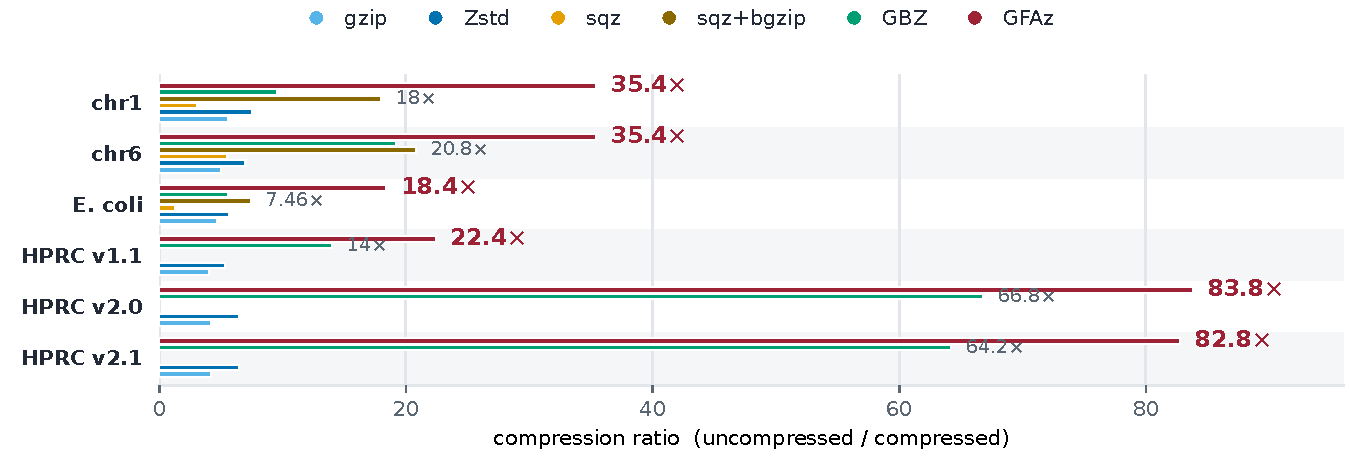
\includegraphics[width=0.63\linewidth]{cpu_ratio.pdf}\\[-0.02cm]

  \begin{minipage}[t]{0.49\linewidth}\centering
    {\large\bfseries\color{slate} Compression throughput}\\[-0.04cm]
    \includegraphics[width=\linewidth]{cpu_compression.pdf}
  \end{minipage}\hfill
  \begin{minipage}[t]{0.49\linewidth}\centering
    {\large\bfseries\color{slate} Decompression throughput}\\[-0.04cm]
    \includegraphics[width=\linewidth]{cpu_decompression.pdf}
  \end{minipage}

  \cpt{Current README results, CPU only. Ratio is uncompressed size / compressed
  size; higher is better. GFAz uses 32 threads, and compression is end-to-end CLI
  wall time. \hd{GFAz reaches 1.36\,GiB/s compression and 5.4\,GiB/s streaming
  decompression while retaining the best ratio on every graph.}}
\end{block}

\end{column}

% ============================== COLUMN 2 =====================================
\begin{column}{0.489\linewidth}

\partbanner{2}{Compute engine}{run the analysis \emph{on} the compressed container}

\begin{block}{}
  \centering
  {\Large\bfseries\color{slate} From compressed paths to analysis results}\\[0.38cm]
  \begin{tikzpicture}[
      font=\small,node distance=7mm,
      stage/.style={draw=rule,line width=2pt,rounded corners=9pt,fill=white,
                    text width=9.65cm,minimum height=7.15cm,align=center,inner sep=5mm},
      ar/.style={-{Stealth[length=5mm,width=4mm]},line width=2.7pt,color=slate},
    ]
    \node[stage,draw=cherry,fill=palec] (packed)
      {{\scriptsize\bfseries\color{cherry}COMPRESSED}\\[0.45cm]
       {\Large\bfseries\color{cherry}\code{.gfaz}}\\[0.35cm]
       grammar-coded paths\\typed columns};
    \node[stage,draw=teal,fill=palet,right=of packed] (extract)
      {{\scriptsize\bfseries\color{teal}FAST PATH EXTRACT}\\[0.45cm]
       {\normalsize\bfseries compact offsets}\\[0.35cm]
       chosen slice\\$12\;\;{-7}\;\;31\;\;8\;\;\cdots$};
    \node[stage,draw=teal,fill=palet,right=of extract] (compute)
      {{\scriptsize\bfseries\color{teal}INDEXED COMPUTE}\\[0.42cm]
       {\scriptsize\bfseries NAME \;|\; GROUP \;|\; OFFSET}\\[0.38cm]
       {\small\bfseries stream visitor}\\compact state};
    \node[stage,draw=cherry,fill=palec,right=of compute] (result)
      {{\scriptsize\bfseries\color{cherry}RESULT}\\[0.48cm]
       {\normalsize\bfseries VCF variants}\\[0.18cm]
       {\normalsize\bfseries TSV matrices}\\[0.18cm]
       curves + statistics};

    \draw[ar] (packed) -- (extract);
    \draw[ar] (extract) -- (compute);
    \draw[ar] (compute) -- (result);

    \coordinate (flowcenter) at ($(extract.south)!0.5!(compute.south)$);
    \node[fill=teal,text=white,rounded corners=6pt,minimum height=1.65cm,
          text width=45.8cm,align=center,font=\small\bfseries,
          below=8mm of flowcenter] (memory)
      {LOW MEMORY \quad one selected stream $+$ bounded decoder scratch $+$ compact analysis state};
    \node[anchor=north,font=\scriptsize\bfseries,text=cherry,
          below=2mm of memory] (never)
      {UNUSED STREAMS REMAIN COMPRESSED \quad $\cdot$ \quad THE FULL GFA IS NEVER MATERIALIZED};
  \end{tikzpicture}

  \vspace{0.35cm}
  \cpt{\code{StreamDecodedNodes} expands a chosen slice and immediately invokes
  the analysis visitor for each signed node. \hd{Only streams used by the query
  are expanded}; they are consumed online rather than retained as decoded paths.}
\end{block}

\gap

\begin{block}{}
  \centering
  {\small
  \setlength{\tabcolsep}{9pt}\renewcommand{\arraystretch}{1.18}
  \begin{tabular}{llcl}
    \toprule
    \textbf{\gz{} command} & \textbf{Reproduces} & \textbf{Passes} & \textbf{Accumulator} \\
    \midrule
    \code{deconstruct} & \code{vg deconstruct}  & 1\,(+topo) & per-site allele table \\
    \code{growth}      & Panacus                & 1          & coverage $\to$ histogram \\
    \code{depth}       & \code{odgi depth}      & 1          & per-node counters \\
    \code{stats}       & \code{odgi stats}      & 0          & metadata totals \\
    \code{pav}         & \code{odgi pav}        & 3          & node$\to$groups CSR \\
    \code{similarity}  & \code{odgi similarity} & 2\,(+join) & node$\to$groups CSR \\
    \bottomrule
  \end{tabular}}
  \cpt{Six analyses, one decoder --- they differ only in the accumulator. A new
  analysis is a new visitor.}
\end{block}

\gap

\begin{block}{}
  \centering
  {\large\bfseries\color{cherry}\code{deconstruct}: GFA\,$\rightarrow$\,VCF with no graph}\\[0.35cm]
  \begin{tikzpicture}[
      >={Stealth[length=4mm]},
      seg/.style={draw,rounded corners=4pt,line width=1.8pt,minimum width=1.9cm,
                  minimum height=1.9cm,inner sep=2pt,align=center,font=\small\ttfamily},
      refp/.style={->,line width=2.4pt,color=cherry},
      altp/.style={->,line width=2.4pt,dashed,color=teal},
    ]
    \node[seg,fill=paleg] (A) at (0,0)      {A\\GAT};
    \node[seg,fill=palet] (B) at (3.4,2.0)  {B\\T};
    \node[seg,fill=palec] (C) at (3.4,-2.0) {C\\C};
    \node[seg,fill=paleg] (D) at (6.8,0)    {D\\GA};
    \node[seg,fill=palec] (E) at (10.2,2.0) {E\\CC};
    \node[seg,fill=paleg] (G) at (13.6,0)   {G\\TT};
    \draw[refp] (A) -- (C); \draw[refp] (C) -- (D);
    \draw[refp] (D) -- (E); \draw[refp] (E) -- (G);
    \draw[altp] (A) -- (B); \draw[altp] (B) -- (D);
    \draw[altp] (D) -- (G);
    \begin{scope}[on background layer]
      \node[draw=slate,dotted,line width=2pt,rounded corners,fit=(B)(C),inner sep=6mm] {};
      \node[draw=slate,dotted,line width=2pt,rounded corners,fit=(E),inner sep=6mm] {};
    \end{scope}
    \node[font=\small,color=slate] at (3.4,4.4)  {snarl $[A,D]$};
    \node[font=\small,color=slate] at (10.2,4.4) {snarl $[D,G]$};
    \node[font=\small,color=cherry,anchor=west] at (0.2,-4.2) {\textbf{---} reference / $h_1$};
    \node[font=\small,color=teal,anchor=west]   at (8.6,-4.2) {\textbf{-\,-} $h_2$};
  \end{tikzpicture}

  \vspace{0.5cm}
  {\small\ttfamily
  \setlength{\tabcolsep}{8pt}\renewcommand{\arraystretch}{1.16}
  \begin{tabular}{llllll}
    \toprule
    \#CHROM & POS & REF & ALT & INFO & h1\ \ h2 \\
    \midrule
    chr1 & 4 & C   & T & AC=1;AN=2;AF=0.5 & 0\ \ \ \ 1 \\
    chr1 & 6 & ACC & A & AC=1;AN=2;AF=0.5 & 0\ \ \ \ 1 \\
    \bottomrule
  \end{tabular}}

  \cpt{\hd{Phase 1} recovers snarls from \emph{topology alone}
  (biconnected decomposition, $O(V{+}E)$, decodes zero haplotypes). \hd{Phase 2}
  streams each haplotype once through a boundary state machine; a reverse boundary
  pair normalizes inversions. No graph, no general snarl index.}
\end{block}

\gap

\begin{block}{}
  \centering
  {\small
  \setlength{\tabcolsep}{6pt}\renewcommand{\arraystretch}{1.20}
  \begin{tabular}{llrrcc}
    \toprule
    \textbf{Analysis} & \textbf{Graph} & \textbf{Baseline} & \textbf{\gz} &
    \textbf{Speedup} & \textbf{Mem.} \\
    \midrule
    \multirow{2}{*}{\code{deconstruct}} & chr1   & 805\,s / 30.3\,GB    & 11.3\,s / 8.3\,GB   & \best\textbf{71$\times$}  & \best\textbf{3.7$\times$} \\
    \emph{vs.} \code{vg}                & HGSVC3 & 132.9\,min / 397\,GB & 8.7\,min / 51.9\,GB & \best\textbf{15$\times$}  & \best\textbf{7.6$\times$} \\
    \midrule
    \multirow{2}{*}{\code{growth}}      & chr1 & 18.3\,s / 6.16\,GB & 0.74\,s / 0.66\,GB & \best\textbf{25$\times$}  & \best\textbf{9.3$\times$} \\
    \emph{vs.} Panacus                  & v2.0 & 245\,min / 327\,GB & 39.8\,s / 12.9\,GB & \best\textbf{369$\times$} & \best\textbf{25$\times$} \\
    \midrule
    \multirow{2}{*}{\code{pav}}         & chr1 & 3499\,s / 31.9\,GB & 11.7\,s / 9.5\,GB & \best\textbf{299$\times$} & \best\textbf{3.4$\times$} \\
    \emph{vs.} \code{odgi}              & chr6 & 4759\,s / 19.4\,GB & 7.8\,s / 6.4\,GB  & \best\textbf{619$\times$} & \best\textbf{3.0$\times$} \\
    \bottomrule
  \end{tabular}}
  \cpt{Wall-clock / peak RSS at 16 threads. \hd{Outputs match the
  baselines:} \code{growth} reproduces Panacus' curve exactly, \code{deconstruct}
  agrees with \code{vg} to within 0.2\% of records, \code{pav} matrices are
  structurally identical to \code{odgi}'s. On the 358/369\,GB HPRC graphs
  \code{vg} and \code{odgi} \emph{cannot load the input at all} --- \gz{} runs
  from a 4.5\,GB container.}
\end{block}

\gap

\begin{block}{}
  \begin{tikzpicture}
    \node[fill=palet,draw=teal,line width=2.5pt,rounded corners=8pt,inner sep=14pt,
          text width=\dimexpr\linewidth-42pt\relax,align=left]{%
      \color{slate}
      \textbf{\large What we built with \gz{}}\\[0.28cm]
      \begin{itemize}
        \item A \hd{state-of-the-art lossless GFA compressor}: 84$\times$ smaller,
              with 1.36/5.43\,GiB/s CPU compression/decompression.
        \item A \hd{compressed-graph compute engine} that uses compact indices and
              expands only selected path streams---never the full GFA.
        \item \hd{Six exact pangenome analyses} running up to
              \textbf{619$\times$ faster} with up to \textbf{25$\times$ less memory}.
      \end{itemize}};
  \end{tikzpicture}
\end{block}

\end{column}
\end{columns}
\end{minipage}

% =============================================================================
%  FOOTER
% =============================================================================
\vfill
\begin{center}
\begin{tikzpicture}
  \node[fill=slate,rounded corners=10pt,inner sep=18pt]{
  \begin{minipage}{0.945\paperwidth}
    \color{white}\small
    \begin{minipage}[c]{0.115\linewidth}
      \centering\colorbox{white}{\color{black}\qrcode[height=5.0cm]{https://github.com/babyplutokurt/GFAz}}\\[3pt]
      {\footnotesize code}
    \end{minipage}\hfill
    \begin{minipage}[c]{0.65\linewidth}
      \textbf{Open source:} \code{github.com/babyplutokurt/GFAz} \ \ $\cdot$ \ \
      \textbf{Contact:} \code{taolue.yang@temple.edu}\\[0.3cm]
      \textbf{Paper:} Yang, Liu, Jiang, Shi, Jin. \emph{\gz{}: Order-of-Magnitude
      Pangenome Analytics by Computing over Compression.} ICS~'26.
      \code{doi:10.1145/3797905.3807870}\\[0.3cm]
      {\footnotesize \textbf{Acknowledgments:} We thank the Human Pangenome Reference
      Consortium (BioProject PRJNA730823) and its funder, NHGRI. Supported in part by
      NIH award R01GM157443.}
    \end{minipage}\hfill
    \begin{minipage}[c]{0.115\linewidth}
      \centering\colorbox{white}{\color{black}\qrcode[height=5.0cm]{https://doi.org/10.1145/3797905.3807870}}\\[3pt]
      {\footnotesize paper}
    \end{minipage}
  \end{minipage}};
\end{tikzpicture}
\end{center}

\end{frame}
\end{document}
